\documentclass{beamer}
\usetheme{Darmstadt}
\usecolortheme{beaver}
\useinnertheme{rectangles}
\setbeamertemplate{footline}[frame number]

\usepackage{lmodern}
\usepackage{natbib}
\usepackage{physics}
\usepackage{siunitx}
\usepackage{xcolor}
\usepackage{graphicx}
\usepackage{bbold}
\usepackage{mathtools}
\usepackage[compat=1.0.0]{tikz-feynman}
\usepackage{physics}

\definecolor{links}{HTML}{2A1B81}
\hypersetup{colorlinks,linkcolor=,urlcolor=links, citecolor=gray}

\usepackage{appendixnumberbeamer}
% \usepackage{hyperref}

% make bibliography entries smaller
\renewcommand\bibfont{\scriptsize}
% If you have more than one page of references, you want to tell beamer
% to put the continuation section label from the second slide onwards
\setbeamertemplate{frametitle continuation}[from second]
% Now get rid of all the colours
\setbeamercolor*{bibliography entry title}{fg=black}
\setbeamercolor*{bibliography entry author}{fg=black}
\setbeamercolor*{bibliography entry location}{fg=black}
\setbeamercolor*{bibliography entry note}{fg=black}
% and kill the abominable icon
\setbeamertemplate{bibliography item}{}

% kill tooltips
\setbeamertemplate{navigation symbols}{}

% \usepackage{beamerthemesplit} // Activate for custom appearance

\newcommand{\zcut}{z_\mathrm{cut}}

\title{Groomed heavy hemisphere mass in $e^+ e^- \to \text{jets}$ events}
\author{Kees Benkendorfer}
\institute{Reed College}
% \institute{UM-CERN REU Final Presentation}
\date{8 December 2020 \\ Thesis Mini-Orals}
% \titlegraphic{\includegraphics[width=0.25\textwidth]{logos/reed_logo.jpg}}

\begin{document}

\begin{frame}[noframenumbering]
	\thispagestyle{empty}
	\titlepage
\end{frame}

\section[Outline]{}
\frame{\tableofcontents}

\section{Background}
\subsection{Events of interest}
	\begin{frame}
		\frametitle{Electron-positron annihilation}
		\begin{columns}
		\column{0.6\textwidth}
		\begin{itemize}
			\item Electron-positron annihilation experiments enable precision probes of the Standard Model
			\begin{itemize}
				\item Theoretically simpler than proton-proton collisions (as at the LHC)

				\item Some results carry over to $pp$ collisions
			\end{itemize}

			\item In events of interest, $e^+$ and $e^-$ produce a photon, which splits into a quark-antiquark pair

			\item One or more gluons are produced off of $q$ or $\bar q$
		\end{itemize}

		\column{0.4\textwidth}
		\begin{figure}
			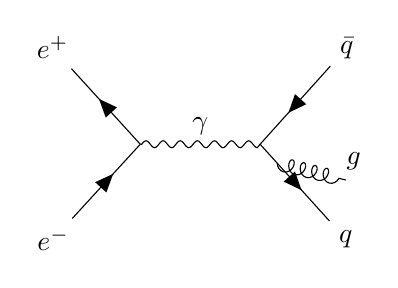
\begin{tikzpicture}
			\begin{feynman}
				\diagram [horizontal=a to b] {
	  				i1 [particle=\(e^{-}\)] -- [fermion] a -- [fermion] i2 [particle=\(e^{+}\)],
	  				a -- [photon, edge label=\(\gamma\)] b,
	  				f1 [particle=\(\bar q\)] -- [fermion] b -- [fermion] f2 [particle=\(q\)],
				};

				\vertex [above = 0.75cm of f2] (r);
				\vertex [right = 0.1cm of r, label = $g$] (g);
	    		\draw [gluon] ($(f2)!0.8!(b)$) -- (r);
			\end{feynman}
			\end{tikzpicture}

			\caption{Feynman diagram for $e^+ e^- \to q\bar q g$}
		\end{figure}
		\end{columns}
	\end{frame}

	\begin{frame}
		\frametitle{Jets}

		\begin{columns}
		\column{0.6\textwidth}
		\begin{itemize}
			\item In quantum chromodynamics (QCD), the gluon carries color charge just like quarks

			\item Interesting nonlinear dynamics:
			\begin{itemize}
				\item \textbf{Self-coupling}: gluons beget gluons

				\item \textbf{Scale-invariance}: QCD events have approximately no intrinsic scale

				\item \textbf{Confinement}: particles with color charge don't like to live alone
			\end{itemize}

			\item Result: producing a quark or gluon yields a collimated spray of hadronic radiation called a \textbf{jet}
		\end{itemize}

		\column{0.4\textwidth}
		\begin{figure}
			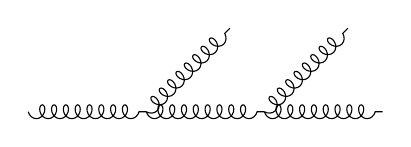
\begin{tikzpicture}
			\begin{feynman}
				\diagram [layered layout, horizontal=a to b] {
	  				a -- [gluon] b -- [gluon] c -- [gluon] d,
				};
				\vertex [above right = of b] (q);
				\vertex [above right = of c] (r);
	    		% \draw [gluon] ($(f2)!0.8!(b)$) -- (r);
	    		\draw [gluon] (b) -- (q);
	    		\draw [gluon] (c) -- (r);
			\end{feynman}
			\end{tikzpicture}

			\caption{QCD self-coupling as gluon propagates}
		\end{figure}
		\end{columns}
	\end{frame}

\subsection{Observables}
	\begin{frame}
		\frametitle{Heavy hemisphere mass}

		\begin{itemize}
			\item We are interested in properties of these jets

			\item Key observable: \textbf{heavy hemisphere mass}
			\begin{itemize}
				\item Split the $e^+ e^- \to \text{jets}$ events into two hemispheres

				\item Look at the normalized mass of the heaviest hemisphere
				
			\end{itemize}

			\item For a heavy hemisphere with four-momentum $P^\mu$, hemisphere mass is given by
			\begin{equation*}
				\rho = \frac{m_h^2}{E_h^2}
			\end{equation*}
			with $m_h^2 = P \cdot P$ and $E_h^2 = \qty(P^0)^2$.
		\end{itemize}
	\end{frame}

	\begin{frame}
		\frametitle{Grooming}

		\begin{itemize}
			\item We almost have a good quantity to measure in experiments

			\item Problem: in high-luminosity colliders, significant background radiation can contaminate jets

			\item This contamination is almost exclusively low-energy (\textbf{soft})

			\item \textbf{Jet grooming}: removes soft emissions in the jet in order to focus on features of interest
			
			\item We use \textbf{mMDT} (modified Mass Drop Tagger) grooming \cite{dasgupta_towards_2013,kardos_two-_2020}
			\begin{itemize}
				\item Set a cutoff energy fraction $\zcut$

				\item For two emissions $i$ and $j$, only keep them if their energies satisfy
				\begin{equation*}
					\frac{\min[E_i, E_j]}{E_i + E_j} > \zcut.
				\end{equation*}
			\end{itemize}
		\end{itemize}
	\end{frame}

\section{Work so far}
\subsection{First-order calculation}
	\begin{frame}
		\frametitle{Reproduction of first-order calculation}

		\begin{itemize}
			% \item QCD calculations must proceed perturbatively

			\item To leading order, $\rho$ is generated by $e^+ e^- \to q \bar q g$ events. For momenta $p_i$ and total momentum $Q$, introduce phase space variables
			\begin{equation*}
				x_i = \frac{2p_i \cdot Q}{Q^2}
			\end{equation*}

			\item With $\alpha_s$ the strong coupling, $C_F = 4/3$ the fundamental Casimir of color, and $\sigma_0$ the cross section for $e^+ e^- \to q\bar q$ events, the cross section is given by \cite{larkoski_improving_2020}:
		\end{itemize}

		\begin{equation*}
			\begin{aligned}
				\frac{1}{\sigma_0}\frac{d\sigma}{d\rho} = \frac{\alpha_s C_F}{2\pi}\int_0^1 &dx_1 \int_0^1 dx_2\,\overbrace{\Theta(x_1 + x_2 - 1)}^{\text{kinematic requirement}} \overbrace{\frac{x_1^2 + x_2^2}{(1 - x_1)(1 - x_2)}}^{\text{matrix element}} \\
					&\times \underbrace{\delta\qty(\rho - \frac{4(1 - \max\qty{x_i})}{(2 - \max\qty{x_i})^2})}_{\text{measurement}} \underbrace{\Theta\qty(\frac{\min\qty{x_i}}{2 - \max\qty{x_i}} - \zcut)}_{\text{jet grooming}}
			\end{aligned}
			\end{equation*}
	\end{frame}

	\begin{frame}
		\frametitle{Reproduction of first-order calculation}

		\begin{figure}
			\includegraphics[width=\columnwidth]{figures/first_reproduction.pdf}

			\caption{Groomed heavy hemisphere mass to first order. Note the cusp around $\rho \sim \zcut$}
		\end{figure}
	\end{frame}

\subsection{Zooming in on intermediate mass}
	\begin{frame}
		\frametitle{Cusp physics}

		\begin{block}{Goal}
			Understand the cusp by performing an all-orders calculation of the distribution in that regime
		\end{block}

		\begin{itemize}
			\item Suppose there are many labeled emissions with energy fractions $z_i$ and angles $\theta_{ij}$

			\item Emissions relevant for the cusp have $z_i \sim \rho$ and $z_i \sim \zcut$. Assuming $\zcut \ll 1$, this means $z_i \ll 1$ (so the emission is soft)

			\item Since $\rho \simeq \sum_{i,j} z_i z_j \theta_{ij}^2$, the leading contribution from emission $i$ will be its interaction with the \textbf{hard} (high-energy) quark $j$, so that $\rho \sim z_i \theta_{ij}^2$

			\item Therefore, $\rho \sim \zcut \theta_{ij}^2 \sim \zcut$, so $\theta_{ij} \sim 1$

			\item Thus, we are looking for \textbf{soft emissions at a wide angle to the quark}
		\end{itemize}
	\end{frame}

	\begin{frame}
		\frametitle{Soft limit}

		\begin{itemize}
			\item In the limit of soft gluon emissions, the matrix element is known \cite{catani_infrared_2000} 

			\item For one gluon with momentum $k^\mu$, the matrix element is
			\begin{equation}
				\abs{\mathcal{M}}^2 = 4\pi\alpha_s C_F \frac{2}{k^+ k^-}
			\end{equation}
			with light-cone coordinates
			\begin{align}
				k^+ &= k^0 - k^3 & k^- &= k^0 + k^3.
			\end{align}

			\item Problem: matrix element diverges in soft limit $k^- \to 0$

			\item Solution: \textbf{dimensional regularization} \cite{schwartz_quantum_2014}
			\begin{itemize}
				\item Basically analytic continuation of the dimension of the problem: work in $d = 4 - 2\epsilon$ dimensions with $\epsilon > 0$

				\item Introduces $(k^+ k^-)^{-\epsilon}$ term which allows integration; also introduces an energy scale $\mu^{2\epsilon}$

				\item Divergences are collected in terms which diverge as $\epsilon \to 0$
			\end{itemize}
		\end{itemize}
	\end{frame}

	\begin{frame}
		\frametitle{Killing divergences}

		\begin{itemize}
			\item Dimensional regularization helps us find divergences --- so what? 
			\begin{itemize}
				\item Divergences remain, only change is they are now explicit

				\item Also, what is $\mu$?
			\end{itemize}

			\item Degeneracy saves the day: adding the remaining singular contributions (i.e., the collinear limit) cancels divergent terms

			\item Can then set $\epsilon = 0$

			\item Adding all degenerate regions of phase space also eliminates terms containing $\mu$
			\begin{itemize}
				\item Physical result must not depend on an arbitrary energy scale
			\end{itemize}
		\end{itemize}
	\end{frame}

	\begin{frame}
		\frametitle{Results: $\zcut = 0.04$}

		\begin{figure}
			\includegraphics[width=\columnwidth]{figures/approximation.pdf}
			\caption{Groomed heavy hemisphere mass to first order, alongside an approximation around the cusp region, with $\zcut = 0.04$}
		\end{figure}
	\end{frame}

	\begin{frame}
		\frametitle{Results: $\zcut = 0.04$}

		\begin{figure}
			\includegraphics[width=\columnwidth]{figures/approximation_zoomed.pdf}
			\caption{Groomed heavy hemisphere mass to first order, alongside an approximation around the cusp region, with $\zcut = 0.04$}
		\end{figure}
	\end{frame}

	\begin{frame}
		\frametitle{Results: $\zcut = 0.001$}

		\begin{figure}
			\includegraphics[width=\columnwidth]{figures/approximation_small_zcut.pdf}
			\caption{Groomed heavy hemisphere mass to first order, alongside an approximation around the cusp region, with $\zcut = 0.001$}
		\end{figure}
	\end{frame}

	\begin{frame}
		\frametitle{Results: $\zcut = 0.001$}

		\begin{figure}
			\includegraphics[width=\columnwidth]{figures/approximation_small_zcut_zoomed.pdf}
			\caption{Groomed heavy hemisphere mass to first order, alongside an approximation around the cusp region, with $\zcut = 0.001$}
		\end{figure}
	\end{frame}


\section{Looking forward}
	\begin{frame}
		\frametitle{Conclusion and next steps}

		\begin{itemize}
			\item I have familiarized myself with previous first-order results
			\begin{itemize}
				\item Has required learning lots of quantum field theory
			\end{itemize}

			\item Main forward thrust will be to derive a new factorization formula describing the distribution to all orders, as in \cite{frye_factorization_2016-1}
			\begin{itemize}
				\item This formula was valid for $\rho \ll \zcut \ll 1$

				\item Factorization formula for $\rho \sim \zcut \ll 1$ would enable calculating the cusp to arbitrary accuracy

				\item The name of the game: ensuring no dependence on arbitrary energy scales $\mu$
			\end{itemize}

			\item With factorization formula in hand, will push to next-order accuracy

			\item Will enable precision understanding of intermediate regions of the distribution
		\end{itemize}
	\end{frame}

\section*{}
    \begin{frame}[allowframebreaks]
        \frametitle{References}
        \bibliographystyle{unsrt}
        %\bibliographystyle{amsalpha}
        \bibliography{jet_substructure}
    \end{frame}

\end{document}
